\subsection{Elettrodo di prima specie}
Gli elettrodi visti finora appartengono a questa categoria. Essi sono metalli immersi in soluzioni dei loro ioni. Si fa ciò per raggiungere molto più velocemente l'equilibrio tra soluzione ed elettrodo, in quanto in acqua l'equilibrio è molto lento perché turbato dalla presenza degli ioni $\rm H_3O^+$.
\subsection{Elettrodo di seconda specie}
\subsection{Elettrodo di terza specie}
\subsection{Elettrodo normale standard ad idrogeno}

\begin{figure}
    \centering
    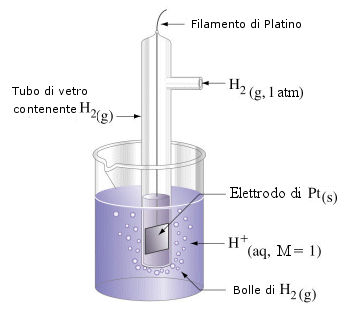
\includegraphics[width=8cm]{immagini/Elettrodo_a_idrogeno.png}
\end{figure}
\subsection{Elettrodo a calomelano saturo}
\begin{figure}
    \centering
    \includegraphics[width=5cm]{immagini/Elettrodo_a_calomelano.png}
\end{figure}
\subsection{Elettrodo d'argento}
\subsection{Elettrodo al chinidrone}
\begin{center}
    \begin{tabular}{p{2.4cm}p{2.5cm}p{2.1cm}p{2cm}}
    \chemfig{*6(-(=O)-=-(=O)-=)} & \vspace{-0.8cm}$\rm + \; 2H^+ \; + \; 2e^-$ & \vspace{-0.9cm} \schemestart \arrow{<=>}      \schemestop &
    \chemfig{*6(=(-OH)-=-(-OH)=-)}\\
    \vspace{0.2cm}\hspace{-0.1cm}Benzochinone & & & \vspace{0.2cm}Idrochinone
    \end{tabular}
\end{center}